% $Header: /cvsroot/latex-beamer/latex-beamer/solutions/conference-talks/conference-ornate-20min.en.tex,v 1.6 2004/10/07 20:53:08 tantau Exp $

\documentclass{beamer}

% This file is a solution template for:

% - Talk at a conference/colloquium.
% - Talk length is about 20min.
% - Style is ornate.



% Copyright 2004 by Till Tantau <tantau@users.sourceforge.net>.
%
% In principle, this file can be redistributed and/or modified under
% the terms of the GNU Public License, version 2.
%
% However, this file is supposed to be a template to be modified
% for your own needs. For this reason, if you use this file as a
% template and not specifically distribute it as part of a another
% package/program, I grant the extra permission to freely copy and
% modify this file as you see fit and even to delete this copyright
% notice.


\mode<presentation>
{
%  \usetheme{Warsaw}
%  \usetheme{Boadilla}
%  \usetheme{Goettingen}
%  \usetheme{Hannover}
%  \usetheme{Madrid}
%  \usetheme{Marburg}
%  \usetheme{Montpellier}
%  \usetheme{Pittsburgh}
  \usetheme{Hawke}
  % or ...

  \setbeamercovered{transparent}
  % or whatever (possibly just delete it)
}


\usepackage[english]{babel}
% or whatever

\usepackage[latin1]{inputenc}
% or whatever

\usepackage{times}
\usepackage[T1]{fontenc}
% Or whatever. Note that the encoding and the font should match. If T1
% does not look nice, try deleting the line with the fontenc.

\usepackage{multimedia}


%%%%%%
% My Commands
%%%%%%

\newcommand{\ml}{{\sc matlab}}

%%%%

\title[Lecture 10] % (optional, use only with long paper titles)
{Lecture 10 - Stability of iteration methods}

% \subtitle
% {Include Only If Paper Has a Subtitle}

\author[I. Hawke] % (optional, use only with lots of authors)
{I.~Hawke}
% - Give the names in the same order as the appear in the paper.
% - Use the \inst{?} command only if the authors have different
%   affiliation.

\institute[University of Southampton] % (optional, but mostly needed)
{
%  \inst{1}%
  School of Mathematics, \\
  University of Southampton, UK
}
% - Use the \inst command only if there are several affiliations.
% - Keep it simple, no one is interested in your street address.

\date[Semester 1] % (optional, should be abbreviation of conference name)
{MATH3018/6141, Semester 1}
% - Either use conference name or its abbreviation.
% - Not really informative to the audience, more for people (including
%   yourself) who are reading the slides online

\subject{Numerical methods}
% This is only inserted into the PDF information catalog. Can be left
% out.



% If you have a file called "university-logo-filename.xxx", where xxx
% is a graphic format that can be processed by latex or pdflatex,
% resp., then you can add a logo as follows:

\pgfdeclareimage[height=0.5cm]{university-logo}{mathematics_7469}
\logo{\pgfuseimage{university-logo}}



% Delete this, if you do not want the table of contents to pop up at
% the beginning of each subsection:
%  \AtBeginSubsection[]
%  {
%    \begin{frame}<beamer>
%      \frametitle{Outline}
%      \tableofcontents[currentsection,currentsubsection]
%    \end{frame}
%  }
\AtBeginSection[]
{
  \begin{frame}<beamer>
    \frametitle{Outline}
    \tableofcontents[currentsection]
  \end{frame}
}


% If you wish to uncover everything in a step-wise fashion, uncomment
% the following command:

%\beamerdefaultoverlayspecification{<+->}


\begin{document}

\begin{frame}
  \titlepage
\end{frame}


\section{Stability and error propagation}

\subsection{Stability}

\begin{frame}
  \frametitle{The problem with the problem}

  We have been finding the root of $f$: solution to
  \begin{equation*}
    f(x) = 0,
  \end{equation*}
  using sequence $\{x_n\}$ from map $g : x_n \rightarrow x_{n+1}$. Map
  designed such that fixed points of $g$ are roots of $f$. Have only
  considered analytically known functions $f$, maps $g$, and round-off
  error. \pause

  \vspace{1ex}

  What if the error is much larger? E.g.\ $f$ given by numerical
  procedure of limited accuracy. Is the iteration numerically stable? \pause

  \vspace{1ex}

  For the rest of this section, only consider the original fixed
  point map
  \begin{equation*}
    g(x) = x - f(x).
  \end{equation*}

\end{frame}

\begin{frame}
  \frametitle{Stability}

  By \emph{stability}, mean small errors from map have only a small
  effect on the answer. \pause More precise: define map
  \begin{equation*}
    G(x) = g(x) + \delta(x).
  \end{equation*}
  $\delta(x)$ is error in evaluating $g$; $G$ is resulting
  numerical approximation. Resulting sequence is
  \begin{equation*}
    X_{n+1} \equiv G(X_n) = g(X_n) + \delta_n, \quad n = 0, 1, 2,
    \dots
  \end{equation*} \pause

  Do not expect $\{X_n\}$ to converge precisely; may expect ($n \to
  \infty$) $X_n$ approximates root up \emph{maximum} error $\delta$.

\end{frame}

\begin{frame}
  \frametitle{Example}

  \begin{overlayarea}{\textwidth}{0.9\textheight}
    \only<1|handout:1>
    {
      \begin{center}
        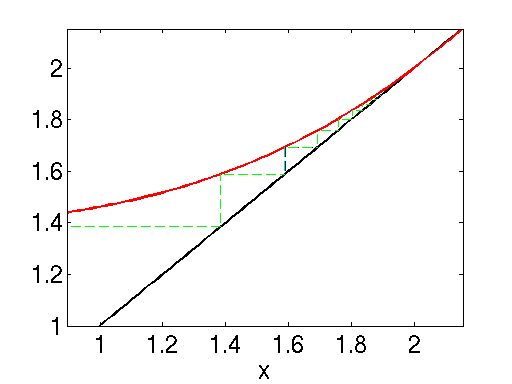
\includegraphics[height=0.8\textheight]{figures/ErrorExample1}
      \end{center}
      With $\delta \sim 10^{-3}$ this example is stable.
    }
    \only<2|handout:2>
    {
      \begin{center}
        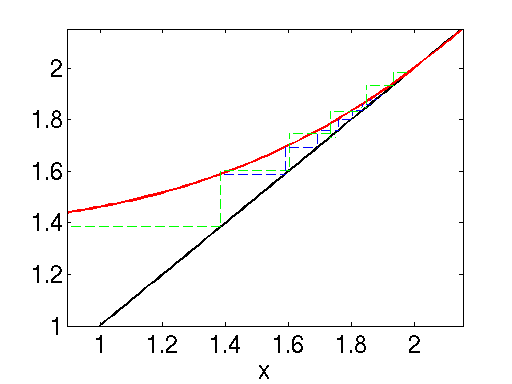
\includegraphics[height=0.8\textheight]{figures/ErrorExample2c}
      \end{center}
      With $\delta \sim 10^{-1}$ this example is unstable.
    }
    \only<3|handout:3>
    {
      \begin{center}
        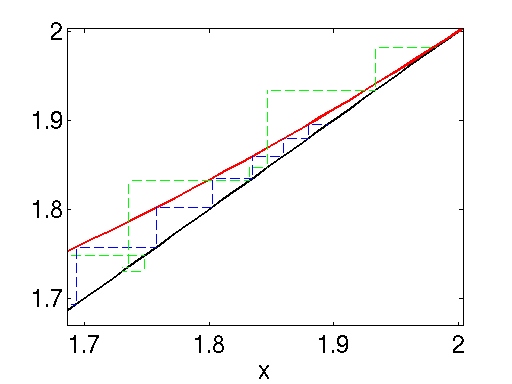
\includegraphics[height=0.8\textheight]{figures/ErrorExample2d}
      \end{center}
      A close up of the random behaviour.
    }
  \end{overlayarea}

\end{frame}


\subsection{Error propagation}


\begin{frame}
  \frametitle{The error band}

  \begin{center}
    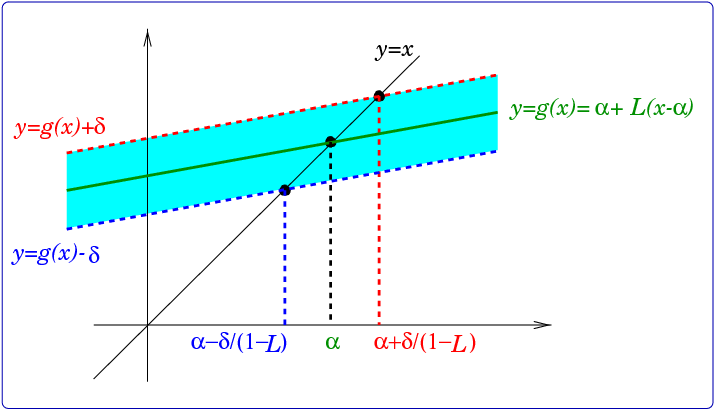
\includegraphics[height=0.7\textheight]{figures/contract_error}
  \end{center}
  If error in evaluating $g$ is bounded by $|\delta_n| \leq \delta
  \,\,\, \forall n$ then error finding $x_{n+1}$ depends on $\delta$
  and slope $L$.

\end{frame}

\begin{frame}
  \frametitle{Theorem}

  Original convergence theorem bounded error $e_n = x_n - s$ as
  \begin{equation*}
    |e_n| \leq \frac{L^n}{1 - L} |x_0 - x_1|.
  \end{equation*} \pause
  For new sequence define $E_n = X_n - s$: bound the error by
  \begin{equation*}
    |E_n| \leq L^n \left(R_0 - \frac{\delta}{1-L} \right) +
    \frac{\delta}{1-L}.
  \end{equation*}
  $R_0$ is new: depends on a \emph{smaller} interval such
  that $G$ remains a contraction mapping, despite error $\delta$.
  \pause

  \vspace{1ex}

  Key results of this theory are
  \begin{itemize}
  \item Sequence converges provided that $R_0$ exists, and
  \item Best possible error is of order $\delta / (1 - L)$.
  \end{itemize}

\end{frame}

\begin{frame}
  \frametitle{Proof}

  Similar to original proof, but error means $g(I) \subseteq I \nRightarrow G(I) \subseteq I$.

  \vspace{1ex}

  For root $s$ assume there exists interval $I(s, r_0) = [s - r_0, s + r_0] \subseteq I$ on which $g$ contracts, $g \left( I(s, r_0) \right) \subseteq I(s, r_0)$. \pause

  \vspace{1ex}

  As in original proof, use induction, triangle inequality:
  \begin{equation*}
    | s - X_n | \leq | g(s) - g(X_{n-1}) | + \delta \leq \dots \leq
    L^n | s - X_0 | + \frac{1 - L^n}{1 - L} \delta.
  \end{equation*}
  First term identical to original proof. \pause

  \vspace{1ex}

  Finally construct $I(s, r_0)$: show that
  \begin{equation*}
    |s - X_0| \leq R_0 \quad \text{where} \quad 0 < R_0 \leq r_0 -
    \frac{\delta}{1 - L} \quad \implies \quad | s - X_n | \leq r_0.
  \end{equation*}

  % \begin{overlayarea}{\textwidth}{0.9\textheight}
  %   \only<1|handout:1>
  %   {
  %     The proof is similar to that for the proof without the error
  %     terms $\delta_n$, and uses induction to construct the bound. The
  %     key difference is that although $g$ is a contraction map in the
  %     interval $I$,
  %     \begin{equation*}
  %       g\left( I \right) \subseteq    I,
  %     \end{equation*}
  %     $G$ may not be due to the errors. We thus need to
  %     construct an interval $I(s, R_0)$ such that
  %     \begin{equation*}
  %       G\left( I(R_0) \right) \subseteq     I(R_0) \subseteq I.
  %     \end{equation*}
  %   }
  %   \only<2-|handout:2>
  %   {
  %     We can do this, as shown in the notes, if the interval is
  %     symmetric about the root,
  %     \begin{equation*}
  %       I(s, r_0) = [s - r_0, s + r_0],
  %     \end{equation*}
  %     and the map $g$ is contracting inside this interval. Induction and
  %     the triangle inequality then gives
  %     \begin{equation*}
  %       | s - X_n| \leq | g(s) - g(X_{n-1})| + \delta \leq \dots \leq
  %       L^n | s - X_0 | + \frac{1 - L^n}{1 - L} \delta.
  %     \end{equation*}
  %     The first term is identical to the proof without error, as
  %     expected.
  %   }
  %   \only<3|handout:2>
  %   {

  %     Finally the hypothesis
  %     \begin{equation*}
  %       |s - X_0| \leq R_0 \quad \text{where} \quad 0 < R_0 \leq r_0 -
  %       \frac{\delta}{1 - L}
  %     \end{equation*}
  %     is introduced. Provided this holds, then
  %     \begin{equation*}
  %       | s - X_n| \leq r_0
  %     \end{equation*}
  %     and the map $G$ does map $I(s, r_0)$ into itself.
  %   }
  % \end{overlayarea}

\end{frame}

\section{Summary}


\subsection{Summary}

\begin{frame}
  \frametitle{Summary}

  \begin{itemize}
  \item The introduction of numerical error (e.g.\ by only knowing
    $f(x)$ to limited precision) affects the stability of the fixed
    point iteration methods.
  \item If the error at any stage $\delta_n$ is bounded by $\delta$, then
    \begin{itemize}
    \item The cumulative error expected is $\delta / (1 - L)$
    \item The initial guess must be within $[s - R_0, s + R_0]$ where
      $R_0$ is defined by
      \begin{enumerate}
      \item The interval within which $g$ is a contracting map, $[s -
        r_0, s + r_0]$, and
      \item The error $\delta$ and Lipschitz constant $L$, as
      \end{enumerate}
      \begin{equation*}
        0 < R_0 \leq r_0 - \frac{\delta}{1-L}.
      \end{equation*}
    \end{itemize}
  \item The proof of convergence is similar to the one without
    numerical error, but care must be taken over the interval to
    ensure that the \emph{numerical} map $G$ does not map points
    outside the interval where the \emph{analytical} map $g$ is
    contracting.
  \end{itemize}

\end{frame}

\end{document}



%%% Local Variables:
%%% mode: latex
%%% TeX-master: t
%%% End:
